\subsection{¿Que es Calibración?}
	\par 
		La palabra "calibración" tiene diferentes significados dependiendo de la industria o el entorno en el que se utiliza. En la industria de prueba y medición, la calibración tiene un significado específico, que, en un nivel básico, es el acto de comparar un dispositivo bajo prueba (DUT por sus siglas en ingles) de un valor desconocido con un estándar de referencia de un valor conocido. Una persona típicamente realiza una calibración para determinar el error o verificar la exactitud del valor desconocido del DUT. Como ejemplo básico, puede realizar una calibración midiendo la temperatura de un termómetro DUT en agua en el punto de ebullición conocido (100 grados Celsius) para conocer el error del termómetro. Debido a que la determinación visual del momento exacto en que se alcanza el punto de ebullición puede ser impreciso, usted puede lograr un resultado más preciso colocando un termómetro de referencia calibrado, de un valor conocido preciso, en el agua para verificar el termómetro DUT.
	
	\par \noindent
		Un siguiente paso lógico que puede ocurrir en un proceso de calibración puede ser ajustar o realzar el instrumento para reducir el error de medición. Técnicamente, el ajuste es un paso separado de la calibración.
		
	\subsubsection{Sistema Internacional de Unidades (SI)}
		\par 
			¿Cómo llegamos a estándares de medición de valores conocidos contra los cuales calibramos nuestros dispositivos bajo prueba? Para la respuesta, pasamos al Sistema Internacional de Unidades, abreviado "SI". El SI consta de siete unidades base que son
			
		\begin{itemize}
			\item  Metro (m): Es la longitud del camino recorrido por la luz en el vacío durante un intervalo de tiempo de 1/299 792 458 de segundo.
			
			\item Kilogramo (kg): Es la unidad de masa; es igual a la masa del prototipo internacional del kilogramo. Actualmente esta siendo redefinida utilizando la balanza de Kibble.
			
			\item Segundo (s): Es la duración de 9 192 631 770 períodos de la radiación correspondiente a la transición entre los dos niveles hiperfinos del estado fundamental del átomo de cesio 133.
			
\clearpage
\thispagestyle{plain}

			\item Ampere (A): Es la corriente constante que, si se mantiene en dos conductores paralelos rectas de longitud infinita, de sección transversal circular insignificante, y se coloca a 1 m de distancia en el vacío, produciría entre estos conductores una fuerza igual a 2 x 10-7 newton por metro de longitud.
			
			\item Kelvin (K): Unidad de temperatura termodinámica, es la fracción 1 / 273.16 de la temperatura termodinámica del punto triple del agua.
			
			\item Mol (mol): Es la cantidad de sustancia de un sistema que contiene tantas entidades elementales como átomos hay en 0.012 kilogramos de carbono 12.
			
			\item Candela (cd): Es la intensidad luminosa, en una dirección dada, de una fuente que emite radiación monocromática de frecuencia 540 x 1012 hercios y que tiene una intensidad radiante en esa dirección de 1/683 vatios por estereorradián.
		\end{itemize}
		
	\subsubsection{Piramide de Trazabilidad de Calibración}
		\par 
			Ahora que tenemos los estándares de referencia SI, ¿cómo los compartimos de manera eficiente y económica con el mundo?
			
		\begin{figure}[h]
			\centering
			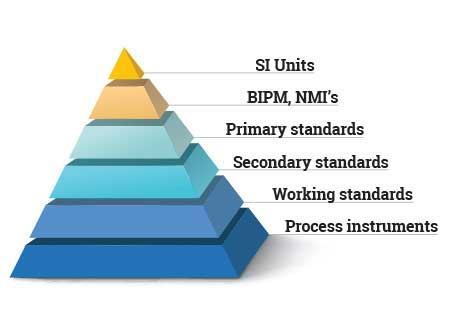
\includegraphics[width=8cm, height=6cm]{piramide.jpg}
			\caption{La Piramide de Trazabilidad de Calibración}
		\end{figure}
		
		\par \noindent
			Piense en el SI en la parte superior de una pirámide de calibración donde el BIPM ayuda a pasar el SI a todos los niveles de uso dentro de los países para fomentar el descubrimiento científico y la innovación, así como la fabricación industrial y el comercio internacional.
			
\clearpage
\thispagestyle{plain}

		\par \noindent 
			Justo debajo del nivel SI, el BIPM (Bureau International des Poinds et Measures por sus siglas en francés), es organización intergubernamental a través de la cual los Estados miembros actúan juntos
			en asuntos relacionados con la ciencia de medición y los estándares de medición, trabaja directamente con los Institutos Nacionales de Metrología (NMIs por sus siglas en inglés) de los estados miembros o países para facilitar la promoción de la SI dentro de esos países.
			
		\par \noindent
			El NMI de los Estados Unidos de América es el National Institute of Standarts and Technology (NIST por sus siglas en inglés); mientras que, el NMI de Panamá es el Centro Nacional de Metrología de Panamá (CENAMEP).
			
		\par \noindent
			Debido a que no es economico, eficiente o incluso posible para todos en un país trabajar directamente con su NMI, los estándares de calibración de NMI se utilizan para calibrar los estándares o instrumentos de calibración primarios; los estándares primarios luego se usan para calibrar estándares secundarios; los estándares secundarios se utilizan para calibrar estándares de trabajo; y los estándares de trabajo se usan para calibrar instrumentos de proceso. De esta manera, las referencias a los estándares SI pueden transmitirse de manera eficiente a través de la NMI a la pirámide de calibración, a la industria según sea necesario.
			
	\subsubsection{Acreditación de Calibración}
		\par 
			Cuando se realizan calibraciones, es importante poder confiar en el proceso por el cual se realizan. La acreditación de calibración brinda esa confianza. La acreditación le da confianza al propietario del instrumento de que la calibración se ha realizado correctamente.
			
		\par \noindent
			La acreditación de calibración significa que se ha revisado un proceso de calibración y se ha encontrado que cumple con los requisitos de metrología técnica y de calidad aceptados internacionalmente. ISO / IEC 17025 es la norma de calidad de metrología internacional a la cual los laboratorios de calibración están acreditados.
			
		\par \noindent
			Los acuerdos internacionales garantizan que una vez que se acredita un proceso de calibración en un país, las calibraciones provenientes de ese proceso pueden aceptarse en todo el mundo sin ningún requisito de aceptación técnica adicional.
			
\clearpage
\thispagestyle{plain}
		
	\subsubsection{Disciplinas de la Calibración}
		\par 
			Hay muchas disciplinas de calibración, cada una con diferentes tipos de calibradores y referencias de calibración. Para tener una idea de los tipos de calibradores e instrumentos que están disponibles. Las disciplinas comunes de calibración incluyen, pero no están limitadas a: electrica, radio frecuencia, temperatura, humedad, presión, flujo de aire, dimensional, tiempo.